% ShortStop, ACIIDS 2027 version (Springer LNCS/LNAI). Build: latexmk -pdf main.tex
% Tables in tables/ are generated by scripts/analyze_calvin_extra.py of the artifact.
\documentclass[runningheads]{llncs}

\usepackage[T1]{fontenc}
\usepackage[utf8]{inputenc}
\usepackage{amsmath,amssymb}
\usepackage{graphicx}
\usepackage{booktabs}
\usepackage{multirow}
\usepackage{array}
\usepackage{xcolor}
\usepackage{tikz}
\usetikzlibrary{arrows.meta,positioning,fit,calc,shapes.geometric,decorations.pathreplacing,matrix}
\usepackage{pgfplots}
\pgfplotsset{compat=1.17}
\usepackage{cite}
\usepackage{orcidlink}
\usepackage{hyperref}
\hypersetup{colorlinks=true,linkcolor=blue!55!black,citecolor=blue!55!black,urlcolor=blue!55!black}

% LNCS float spacing is generous; tighten it slightly.
\setlength{\textfloatsep}{10pt plus 2pt minus 2pt}
\setlength{\intextsep}{10pt plus 2pt minus 2pt}
\setlength{\floatsep}{8pt plus 2pt minus 2pt}
\setlength{\abovecaptionskip}{5pt}
\renewcommand{\topfraction}{0.85}
\renewcommand{\textfraction}{0.1}
\setcounter{topnumber}{3}
\raggedbottom
\clubpenalty=300
\widowpenalty=300

\spnewtheorem{assumption}{Assumption}{\bfseries}{\itshape}

\newcommand{\sys}{\textsc{ShortStop}}
\newcommand{\Rh}{\hat{\mathcal{R}}}
\newcommand{\Xu}{\mathcal{X}_u}
\newcommand{\Xs}{\mathcal{X}_s}
\newcommand{\fhat}{\hat{f}}
% Expandable \input (primitive) so generated rows can sit between booktabs rules.
\makeatletter\newcommand{\tablerows}[1]{\@@input #1 }\makeatother

\begin{document}

\title{Counterexample-Guided Short-Horizon Shielding\texorpdfstring{\\}{ }of Generative Robot Policies}
\titlerunning{Counterexample-Guided Shielding of Generative Robot Policies}

\author{Cong-Tu Le\inst{1}\,\orcidlink{0009-0002-7873-6926} \and Xuan-Bach Le\inst{1}\,\orcidlink{0009-0003-6848-5403}}
\authorrunning{C.-T. Le and X.-B. Le}
\institute{Ho Chi Minh City University of Technology (HCMUT),\\
Vietnam National University Ho Chi Minh City (VNU-HCM), Vietnam\\
\email{congtu305@gmail.com, lexuanbach@hcmut.edu.vn}}

\maketitle

\begin{abstract}
Generative robot policies commit to several future motions at once. An
unfamiliar obstacle can therefore cause a collision before the next policy
query. We present \sys{}, a runtime shield that checks and repairs these
action chunks without retraining the policy. Bands for model error around predicted arm poses form a reachtube.
A lower bound on Signal Temporal Logic (STL) robustness certifies chunks
whose tube--obstacle clearance meets a margin. If all candidates fail,
the point of least clearance guides repair, with joint holding as fallback. Safety depends on tube coverage, for which we
derive a statistical bound. Inference delay requires a certified horizon
$H\ge r+d$, where $r$ steps execute per decision and computation takes
$d$ steps. On CALVIN
(Composing Actions from Language and Vision), a frozen Multimodal Diffusion
Transformer with our shield reduces collisions from 39.7\% to 1.1\% across
1000 pre-registered obstacle scenes. Collision-free task completion rises
from 58.4\% to 80.0\%, comparable to filters sharing our model and margins.
The arm leaves its tube in 0.10\% of 41{,}899 audited steps. With three
steps of inference delay, the extended horizon yields 0.0\% violations,
compared with 31.5\% without delay awareness.

\keywords{Safe robot learning \and Diffusion policy \and Action chunking
\and Reachability \and Signal temporal logic \and Runtime shielding.}
\end{abstract}

%=====================================================================
\section{Introduction}

A robot reaching for a drawer handle may encounter a ball that was absent
from its demonstrations (Fig.~\ref{fig:loop}). If the policy cannot see the
ball, it proposes the familiar approach. Holding the arm avoids a collision
but leaves the drawer closed. To finish the task, the robot must adjust
that approach while preserving its progress toward the handle.

Diffusion models~\cite{chi2023diffusion,janner2022planning} and flow
matching~\cite{lipman2023flow} trained on demonstrations represent several
possible motions for one observation. Both emit \emph{action chunks},
sequences of future actions whose prefix runs before the next policy query.
Chunking improves temporal consistency and throughput~\cite{chi2023diffusion},
but the executed prefix is \emph{open-loop}: the policy cannot revise it
in response to an obstacle. Verifying every possible output would require
reasoning through repeated generative sampling and contact dynamics,
beyond the modest networks and short horizons supported by
neural-network reachability tools~\cite{tran2020nnv,everett2021reachability}.

Once proposed, however, a chunk has fixed actions. Their short-term effects
under model error form a \emph{reachtube} of possible arm positions.
\sys{} sits between policy and robot as a \emph{runtime shield}, checking
this tube against constraints in Signal Temporal Logic (STL). The
\emph{robustness} of a constraint measures its margin of satisfaction.
A failed check pinpoints the band nearest the obstacle. This
\emph{counterexample} guides repair, followed by another check. The loop
draws on counterexample-guided synthesis and
falsification~\cite{solar2006sketching,clarke2000cegar,annpureddy2011staliro}.
The paper makes three contributions.

\begin{itemize}
\item A runtime shield checks and repairs chunks from a frozen generative
policy (Sect.~\ref{sec:method}).
\item The analysis establishes conditional safety, bounds unnecessary
rejection, and derives the certification horizon required under inference delay
(Sect.~\ref{sec:theory}).
\item Evaluation on 1000 pre-registered CALVIN obstacle scenes covers five
baselines, two sharing our model, error bound and margins, with paired
comparisons, an assumption audit, a delay test and ablations
(Sects.~\ref{sec:setup}--\ref{sec:analysis}).
\end{itemize}

\begin{figure}[t]
\centering
% Generated by figures/make_fig1.py. Do not edit by hand.
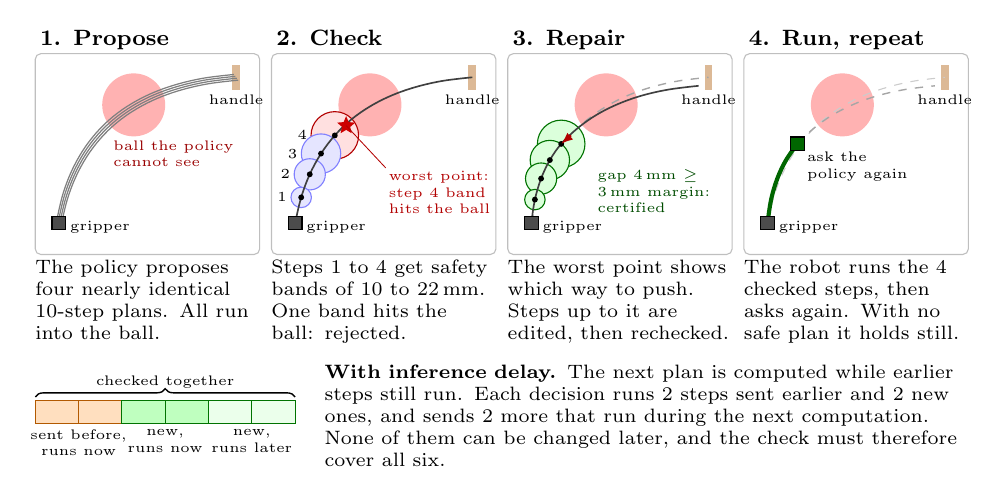
\begin{tikzpicture}[x=1cm,y=1cm,
  frame/.style={draw=black!25, rounded corners=2pt},
  ttl/.style={font=\footnotesize\bfseries, inner sep=1pt},
  lbl/.style={font=\tiny, inner sep=1pt},
  capt/.style={font={\scriptsize\hyphenpenalty10000\exhyphenpenalty10000\relax}, text width=2.85cm, align=left, anchor=north, inner sep=0pt},
  grip/.style={draw=black, fill=black!70, minimum size=5pt, inner sep=0pt, rectangle},
  ballc/.style={red!30},
  badband/.style={fill=red!12, draw=red!70!black, line width=0.4pt},
  band/.style={fill=blue!10, draw=blue!50, line width=0.4pt},
  okband/.style={fill=green!14, draw=green!45!black, line width=0.4pt},
  planline/.style={black!75, line width=0.6pt},
  stepdot/.style={circle, fill=black, inner sep=0.75pt}]
\begin{scope}[xshift=0.00cm]
\draw[frame] (0,0) rectangle (2.85,2.55);
\node[ttl, anchor=base west] at (0.02,2.65) {1. Propose};
\fill[brown!55] (2.500,2.090) rectangle (2.600,2.410);
\node[lbl, anchor=north] at (2.550,2.070) {handle};
\fill[ballc] (1.250,1.900) circle (0.4);
\node[lbl, align=left, text=red!60!black, anchor=west] at (0.950,1.280) {ball the policy\\cannot see};
\draw[black!50, line width=0.45pt] plot[smooth, tension=0.6] coordinates {(0.273,0.436) (0.349,0.761) (0.459,1.054) (0.602,1.317) (0.777,1.548) (0.985,1.749) (1.227,1.918) (1.502,2.057) (1.809,2.164) (2.149,2.241) (2.523,2.286)};
\draw[black!50, line width=0.45pt] plot[smooth, tension=0.6] coordinates {(0.291,0.412) (0.367,0.737) (0.477,1.030) (0.620,1.293) (0.795,1.524) (1.004,1.725) (1.245,1.894) (1.520,2.033) (1.827,2.140) (2.167,2.217) (2.541,2.262)};
\draw[black!50, line width=0.45pt] plot[smooth, tension=0.6] coordinates {(0.309,0.388) (0.386,0.713) (0.495,1.006) (0.638,1.269) (0.813,1.500) (1.021,1.701) (1.263,1.870) (1.538,2.009) (1.845,2.116) (2.185,2.193) (2.559,2.238)};
\draw[black!50, line width=0.45pt] plot[smooth, tension=0.6] coordinates {(0.327,0.364) (0.404,0.689) (0.513,0.982) (0.656,1.245) (0.831,1.476) (1.039,1.677) (1.281,1.846) (1.556,1.985) (1.863,2.092) (2.204,2.169) (2.577,2.214)};
\node[grip] at (0.300,0.400) {};
\node[lbl, anchor=west] at (0.400,0.350) {gripper};
\node[capt] at (1.425,-0.06) {The policy proposes four nearly identical 10-step plans. All run into the ball.};
\end{scope}
\begin{scope}[xshift=3.00cm]
\draw[frame] (0,0) rectangle (2.85,2.55);
\node[ttl, anchor=base west] at (0.02,2.65) {2. Check};
\fill[brown!55] (2.500,2.090) rectangle (2.600,2.410);
\node[lbl, anchor=north] at (2.550,2.070) {handle};
\fill[ballc] (1.250,1.900) circle (0.4);
\draw[badband] (0.804,1.512) circle (0.302);
\draw[band] (0.629,1.281) circle (0.250);
\draw[band] (0.486,1.018) circle (0.198);
\draw[band] (0.377,0.725) circle (0.130);
\draw[planline] plot[smooth, tension=0.6] coordinates {(0.300,0.400) (0.377,0.725) (0.486,1.018) (0.629,1.281) (0.804,1.512) (1.012,1.713) (1.254,1.882) (1.529,2.021) (1.836,2.128) (2.176,2.205) (2.550,2.250)};
\node[stepdot] at (0.377,0.725) {};
\node[lbl, anchor=east] at (0.237,0.725) {1};
\node[stepdot] at (0.486,1.018) {};
\node[lbl, anchor=east] at (0.278,1.018) {2};
\node[stepdot] at (0.629,1.281) {};
\node[lbl, anchor=east] at (0.369,1.281) {3};
\node[stepdot] at (0.804,1.512) {};
\node[lbl, anchor=east] at (0.492,1.512) {4};
\node[star, star points=5, star point ratio=2.2, fill=red!80!black, inner sep=1.1pt] at (0.948,1.637) {};
\draw[red!70!black, line width=0.3pt] (0.948,1.637) -- (1.45,1.10) node[lbl, anchor=north west, align=left, text=red!70!black] {worst point:\\step 4 band\\hits the ball};
\node[grip] at (0.300,0.400) {};
\node[lbl, anchor=west] at (0.400,0.350) {gripper};
\node[capt] at (1.425,-0.06) {Steps 1 to 4 get safety bands of 10 to 22\,mm. One band hits the ball: rejected.};
\end{scope}
\begin{scope}[xshift=6.00cm]
\draw[frame] (0,0) rectangle (2.85,2.55);
\node[ttl, anchor=base west] at (0.02,2.65) {3. Repair};
\fill[brown!55] (2.500,2.090) rectangle (2.600,2.410);
\node[lbl, anchor=north] at (2.550,2.070) {handle};
\fill[ballc] (1.250,1.900) circle (0.4);
\draw[black!35, dashed, line width=0.5pt] plot[smooth, tension=0.6] coordinates {(0.300,0.400) (0.377,0.725) (0.486,1.018) (0.629,1.281) (0.804,1.512) (1.012,1.713) (1.254,1.882) (1.529,2.021) (1.836,2.128) (2.176,2.205) (2.550,2.250)};
\draw[okband] (0.679,1.404) circle (0.302);
\draw[okband] (0.535,1.199) circle (0.250);
\draw[okband] (0.424,0.964) circle (0.198);
\draw[okband] (0.345,0.697) circle (0.130);
\draw[planline] plot[smooth, tension=0.6] coordinates {(0.300,0.400) (0.345,0.697) (0.424,0.964) (0.535,1.199) (0.679,1.404) (0.888,1.604) (1.129,1.774) (1.404,1.912) (1.711,2.020) (2.052,2.096) (2.425,2.142)};
\node[stepdot] at (0.345,0.697) {};
\node[stepdot] at (0.424,0.964) {};
\node[stepdot] at (0.535,1.199) {};
\node[stepdot] at (0.679,1.404) {};
\draw[-{Latex[length=1.5mm]}, red!70!black, line width=0.7pt] (0.804,1.512) -- (0.679,1.404);
\node[lbl, anchor=north west, align=left, text=green!30!black] at (1.10,1.12) {gap 4\,mm $\geq$\\3\,mm margin:\\certified};
\node[grip] at (0.300,0.400) {};
\node[lbl, anchor=west] at (0.400,0.350) {gripper};
\node[capt] at (1.425,-0.06) {The worst point shows which way to push. Steps up to it are edited, then rechecked.};
\end{scope}
\begin{scope}[xshift=9.00cm]
\draw[frame] (0,0) rectangle (2.85,2.55);
\node[ttl, anchor=base west] at (0.02,2.65) {4. Run, repeat};
\fill[brown!55] (2.500,2.090) rectangle (2.600,2.410);
\node[lbl, anchor=north] at (2.550,2.070) {handle};
\fill[ballc] (1.250,1.900) circle (0.4);
\draw[black!20, dashed, line width=0.4pt] plot[smooth, tension=0.6] coordinates {(0.300,0.400) (0.377,0.725) (0.486,1.018) (0.629,1.281) (0.804,1.512) (1.012,1.713) (1.254,1.882) (1.529,2.021) (1.836,2.128) (2.176,2.205) (2.550,2.250)};
\draw[green!40!black, line width=1.5pt] plot[smooth, tension=0.6] coordinates {(0.300,0.400) (0.345,0.697) (0.424,0.964) (0.535,1.199) (0.679,1.404)};
\draw[black!35, dashed, line width=0.5pt] plot[smooth, tension=0.6] coordinates {(0.679,1.404) (0.888,1.604) (1.129,1.774) (1.404,1.912) (1.711,2.020) (2.052,2.096) (2.425,2.142)};
\node[grip, fill=green!40!black] at (0.679,1.404) {};
\node[lbl, anchor=north west, align=left] at (0.759,1.344) {ask the\\policy again};
\node[grip] at (0.300,0.400) {};
\node[lbl, anchor=west] at (0.400,0.350) {gripper};
\node[capt] at (1.425,-0.06) {The robot runs the 4 checked steps, then asks again. With no safe plan it holds still.};
\end{scope}
\draw[fill=orange!25, draw=orange!70!black] (0.00,-2.15) rectangle (0.55,-1.85);
\draw[fill=orange!25, draw=orange!70!black] (0.55,-2.15) rectangle (1.10,-1.85);
\node[lbl, anchor=north, align=center] at (0.55,-2.18) {sent before,\\runs now};
\draw[fill=green!25, draw=green!45!black] (1.10,-2.15) rectangle (1.65,-1.85);
\draw[fill=green!25, draw=green!45!black] (1.65,-2.15) rectangle (2.20,-1.85);
\node[lbl, anchor=north, align=center] at (1.65,-2.18) {new,\\runs now};
\draw[fill=green!8, draw=green!45!black] (2.20,-2.15) rectangle (2.75,-1.85);
\draw[fill=green!8, draw=green!45!black] (2.75,-2.15) rectangle (3.30,-1.85);
\node[lbl, anchor=north, align=center] at (2.75,-2.18) {new,\\runs later};
\draw[decorate, decoration={brace, amplitude=3pt}, line width=0.5pt] (0.00,-1.81) -- (3.30,-1.81) node[midway, above=2pt, lbl] {checked together};
\node[font=\scriptsize, anchor=west, text width=8.2cm, align=left] at (3.55,-2.05) {\textbf{With inference delay.} The next plan is computed while earlier steps still run. Each decision runs 2 steps sent earlier and 2 new ones, and sends 2 more that run during the next computation. None of them can be changed later, and the check must therefore cover all six.};
\end{tikzpicture}

\caption{One \sys{} decision, viewed from above with gripper bands only.
Band widths and margin match the experiments. The scene and gaps are
illustrative. Sections~\ref{sec:method} and~\ref{sec:theory} formalize the steps.}
\label{fig:loop}
\end{figure}

%=====================================================================
\section{Related Work}\label{sec:related}

\textbf{Generative policies.} Diffusion produces action
chunks~\cite{chi2023diffusion,reuss2024mdt} or complete
trajectories~\cite{janner2022planning}. Flow matching generates actions
through an ordinary differential equation~\cite{lipman2023flow}.
Real-time chunking overlaps computation and execution~\cite{black2025rtc}.
Safety can enter generation through constraint
projection~\cite{power2023sampling}, barrier conditions in the
noise-removal network~\cite{xiao2023safediffuser}, or differentiable STL
robustness~\cite{meng2025diverse}. In \sys{}, the safety check follows
generation and leaves the learned policy unchanged.

\textbf{Safety filters.} Shields can override unsafe actions using a
verified state machine~\cite{alshiekh2018shielding}, and safe reinforcement
learning constrains training~\cite{brunke2022safe}. Predictive safety
filters optimize corrections to proposed inputs~\cite{wabersich2021predictive},
and model-predictive shielding switches to a backup
policy~\cite{bastani2021mps}. A control barrier function (CBF) inside a quadratic program (QP) keeps the
state in a safe set~\cite{ames2017cbfqp}, a property called \emph{set
invariance}. Hamilton--Jacobi reachability computes states
from which safety can be maintained~\cite{bansal2017hj}.

Closest to our setting, Reachability-Aided Imitation Learning (RAIL)
filters diffusion actions~\cite{jung2024rail}. PACS, a path-consistent
safety filter, brakes along each generated path and checks its braking
trajectory with reachable sets~\cite{roemer2026pacs}. CBFs in learned
representations filter image-based policies~\cite{nakamura2025latentcbf}, and
multi-link filters protect vision-language-action policies, which map
images and language to actions~\cite{agarwal2026multilink}. Our focus within this setting is tube-based STL certification,
counterexample-guided repair, and the horizon needed when computation
overlaps execution.

\textbf{Reachability, STL and counterexamples.} Set-based motion
bounds~\cite{althoff2015cora} and quantitative STL
semantics~\cite{donze2010robust,fainekos2009robustness} provide the basis
for our online check~\cite{deshmukh2017robust}. Its witness connects
monitoring to chunk revision through
counterexamples~\cite{solar2006sketching,clarke2000cegar,annpureddy2011staliro}.

%=====================================================================
\section{Method}\label{sec:method}

\textbf{Problem setup.} At discrete time $t$, the robot state $x_t$ belongs
to a state space $\mathcal{X}$ and evolves as $x_{t+1}=f(x_t,a_t)+w_t$.
Here $a_t$ is an action, $f$ the unknown dynamics, and $w_t$ a disturbance
with norm bounded by $\bar w$. We write $\|\cdot\|$ for the Euclidean norm.
Our frozen policy $\pi_\theta$, with fixed learned parameters $\theta$,
maps observation $o_t$ to a distribution over action chunks
$a_{t:t+L}=(a_t,\dots,a_{t+L-1})$. The slice excludes its endpoint, giving $L$ \emph{rows}, one action per
step. The shield certifies $H$ rows and executes $r$ before the next
decision, with $r\le H\le L$. For example, Fig.~\ref{fig:loop} proposes ten rows,
checks four, and executes those four.

The experimental STL specification $\varphi$, formalized in (C), requires
avoiding the unsafe set $\Xu$ at steps 1 to $H$. We write
$\mathrm{dist}(x,\Xu)$ for the signed clearance between the arm at state $x$
and the obstacles, negative under penetration.

\textbf{(P) Proposal.} We draw $K$ candidate chunks
$\{a^{(i)}\}_{i=1}^K \sim \pi_\theta(\cdot\mid o_t)$, where $i$ indexes
candidates, in one batched call (Fig.~\ref{fig:loop}, panel~1). Their
task-progress score $g(a)$ is the negative distance from the predicted
end-effector (tool) position after the last row to the current sub-goal.
Chunks that end closer to the goal rank higher. The simulator supplies
the contact point and movement target, such as a drawer's handle and target
opening position. Selection and repair act on chunks while leaving
$\pi_\theta$ unchanged.

\textbf{(R) Short-horizon reachtube.} A band around each predicted arm pose
accounts for prediction error. These sets $\Rh_k$ at future steps $k$
form the tube $\Rh=(\Rh_1,\dots,\Rh_H)$.
Starting from the known state $\Rh_0=\{x_t\}$, we set
\begin{equation}
\Rh_{k} = \fhat_k\!\left(x_t, a_{t:t+k}\right) \oplus \mathcal{B}\!\left(\epsilon_k + \bar w\right), \quad 1 \le k \le H,
\label{eq:tube}
\end{equation}
where $\fhat$ is our approximate dynamics model, $\fhat_k$ its $k$-step
prediction, and $\epsilon_k$ a calibrated bound on the $k$-step error.
The Minkowski sum $\oplus\mathcal{B}(\varrho)$ adds every displacement in
a ball of radius $\varrho$, expanding the prediction into a band.
Because Eq.~\eqref{eq:tube} bounds the full $k$-step deviation directly,
$\epsilon_k$ must also cover accumulated disturbance.
The implementation uses seven joint angles $q\in\mathbb{R}^7$ as its state.
The tool Jacobian maps small joint motions to tool motions. Its damped
least-squares inverse maps requested tool motions back to joint steps
while limiting large updates~\cite{nakamura1986inverse}.
Forward kinematics gives the corresponding arm positions, which we
represent by \emph{capsules}, line segments thickened by a radius. The hand capsule extends from the wrist flange to the tool point
and covers the fingers at any opening. For collision checks, we represent
$\Rh_k$ in physical space by these capsules inflated by
$\epsilon_k+\bar w$ (Fig.~\ref{fig:loop}, panel~2).

\textbf{(C) STL and its robustness over the tube.} STL formulas in negation
normal form follow the grammar
\[
\varphi ::= \mu \mid \neg\mu \mid \varphi_1\wedge\varphi_2 \mid
\varphi_1\vee\varphi_2 \mid \square_I\varphi \mid \lozenge_I\varphi \mid
\varphi_1\,\mathcal{U}_I\,\varphi_2 ,
\]
where a predicate $\mu$ states $h_\mu(x)\ge 0$ for a real function $h_\mu$
of the state, $I=[a,b]$ is an interval of steps with integers
$0\le a\le b$, and $\square$, $\lozenge$ and $\mathcal{U}$ read
``always'', ``eventually'' and ``until''. For a trajectory
$\xi=(\xi_0,\xi_1,\dots)$ with $\xi_0=x_t$, the robustness at step $k$ is
defined recursively~\cite{donze2010robust,fainekos2009robustness}:
\begin{align*}
\rho(\mu,\xi,k)&=h_\mu(\xi_k), &
\rho(\neg\mu,\xi,k)&=-h_\mu(\xi_k),\\
\rho(\varphi_1\wedge\varphi_2,\xi,k)&=\min\nolimits_{j}\rho(\varphi_j,\xi,k), &
\rho(\varphi_1\vee\varphi_2,\xi,k)&=\max\nolimits_{j}\rho(\varphi_j,\xi,k),\\
\rho(\square_I\varphi,\xi,k)&=\min_{k'\in k+I}\rho(\varphi,\xi,k'), &
\rho(\lozenge_I\varphi,\xi,k)&=\max_{k'\in k+I}\rho(\varphi,\xi,k'),
\end{align*}
\[
\rho(\varphi_1\,\mathcal{U}_I\,\varphi_2,\xi,k)=\max_{k'\in k+I}
\min\Big(\rho(\varphi_2,\xi,k'),\ \min_{k\le k''<k'}\rho(\varphi_1,\xi,k'')\Big),
\]
and $\rho(\varphi,\xi)=\rho(\varphi,\xi,0)$. Positive robustness implies
that $\xi$ satisfies $\varphi$, negative robustness implies violation, and
$|\rho|$ measures how far the predicate values are from flipping the
verdict. The interval semantics over a tube replaces each predicate value by
its worst case over the band, $\rho(\mu,\Rh,k)=\inf_{x\in\Rh_k}h_\mu(x)$ and
$\rho(\neg\mu,\Rh,k)=\inf_{x\in\Rh_k}(-h_\mu(x))$, and keeps the other
rules. Because $\min$ and $\max$ are monotone, induction on $\varphi$ gives
$\rho(\varphi,\Rh)\le\rho(\varphi,\xi)$ for every $\xi$ with
$\xi_k\in\Rh_k$, which is Assumption~\ref{as:stl}. Avoidance takes the
predicate $h(x)=\mathrm{dist}(x,\Xu)$ under $\square_{[1,H]}$, and its
tube robustness is
\begin{equation}
\rho(\varphi, \Rh) = \min_{1 \le k \le H}\; \inf_{x \in \Rh_k} \mathrm{dist}(x, \Xu),
\label{eq:rho}
\end{equation}
The infimum finds the least clearance within each band, and the minimum
selects the worst step. Certification requires
$\rho(\varphi,\Rh)\ge\gamma>0$ for a chosen safety margin.
The 4~mm gap in Fig.~\ref{fig:loop}, panel~3, passes our 3~mm margin.
A 2~mm gap would fail despite leaving the nominal motion collision-free.
Capsule--sphere distance has a closed-form expression, making this bound
exact for the tube. Exact distances to other convex obstacles preserve
this property. We evaluate only avoidance, leaving richer temporal
specifications untested.

\textbf{(S) Counterexample-guided repair and selection.} Rejection supplies
more than a verdict. It identifies the worst-case witness
\begin{equation}
(k^\star, x^\star) = \arg\min_{1 \le k \le H,\, x \in \Rh_k} \mathrm{dist}(x, \Xu),
\label{eq:ce}
\end{equation}
the closest point on the inflated arm (the star in Fig.~\ref{fig:loop},
panel~2). If $\rho=\rho(\varphi,\Rh)<\gamma$, the witness is a
counterexample to certification. The gradient
$v=\nabla_{a_{t:t+k^\star}}\mathrm{dist}(x^\star(a),\Xu)$, computed through
the witness point's Jacobian, is the action direction that increases its
clearance. With an extra repair margin $\mu>0$, the Polyak
step~\cite{polyak1969minimization} makes the smallest change satisfying the
linear approximation of the clearance constraint,
\begin{equation}
a_{t:t+k^\star} \leftarrow a_{t:t+k^\star} + \frac{\gamma + \mu - \rho}{\|v\|^2}\, v,
\label{eq:repair}
\end{equation}
for nonzero $v$. The update changes only rows through $k^\star$ (panel~3),
shifting the positions reached by later relative actions as well.
Moving a band can expose a different closest point, requiring a new
witness and a full tube check after each update, for at most
$n_{\mathrm{rep}}$ rounds. If every original candidate fails, repair tries
them in decreasing order of $g(a)$ until one certifies.
Among the available certified chunks, we select
\begin{equation}
a^\star = \arg\max_{a \text{ certified}} g(a)
\label{eq:select}
\end{equation}
and execute its first $r$ rows. If none certifies, our fallback controller
$\pi_{\mathrm{fb}}$ holds the joints for one step before we query the policy
again. Each decision needs $K$ tube checks and at most $K n_{\mathrm{rep}}$
repair rounds.

%=====================================================================
\section{Theory}\label{sec:theory}

\begin{assumption}[Sound tube]\label{as:tube}
For every committed chunk, the states that its first $H$ rows would produce
from $x_t$ satisfy $x_{t+k} \in \Rh_k$ for $1 \le k \le H$.
\end{assumption}
\begin{assumption}[Sound robustness bound]\label{as:stl}
For every tube and every trajectory $\xi$ with $\xi_k \in \Rh_k$ for
$1 \le k \le H$, we have $\rho(\varphi, \Rh) \le \rho(\varphi, \xi)$.
\end{assumption}
\begin{assumption}[Safe fallback]\label{as:fb}
There is a maximum clearance loss $0\le\eta < \gamma$ such that, from any state with
$\mathrm{dist}(x,\Xu) \ge \gamma$, holding with $\pi_{\mathrm{fb}}$ keeps
$\mathrm{dist} \ge \gamma - \eta$ for any number of steps.
\end{assumption}

The induction in Sect.~\ref{sec:method}~(C) establishes
Assumption~\ref{as:stl}. Tube coverage and fallback safety require empirical
evidence, examined in Sect.~\ref{sec:soundness}.

\begin{theorem}[Short-horizon safety]\label{thm:safety}
Let Assumptions~\ref{as:tube} and~\ref{as:stl} hold and let the shield
commit at time $t$ a chunk whose tube $\Rh^\star$ satisfies
$\rho(\varphi, \Rh^\star) \ge \gamma > 0$.
Then each state $x_{t+k}$ with $1 \le k \le H$ that the chunk's first $H$
rows would produce satisfies $\mathrm{dist}(x_{t+k}, \Xu) \ge \gamma$. In particular the
$r \le H$ executed rows keep the arm at least $\gamma$ from $\Xu$.
\end{theorem}
\begin{proof}
Assumption~\ref{as:tube} places the states inside $\Rh^\star$.
Assumption~\ref{as:stl} bounds their robustness below by $\gamma$.
For avoidance, Eq.~\eqref{eq:rho} therefore gives clearance at least
$\gamma$ at every checked step.
The executed prefix has $r\le H$ rows, and repaired chunks pass the
same check. \qed

\end{proof}

\begin{corollary}[All-time safety]\label{cor:alltime}
Suppose Assumptions~\ref{as:tube}--\ref{as:fb} hold, with a sound tube
at every decision. If the initial state $x_0$ satisfies
$\mathrm{dist}(x_0,\Xu)\ge\gamma$, then every state has clearance
$\mathrm{dist}(x_t,\Xu)\ge\gamma-\eta>0$.
\end{corollary}
\begin{proof}
Every executed certified row ends with clearance at least $\gamma$ by
Theorem~\ref{thm:safety}, which does not require the chunk to start from a
safe state. A stall therefore starts with clearance at least $\gamma$, and
Assumption~\ref{as:fb} keeps $\mathrm{dist} \ge \gamma - \eta$ until the next
certified chunk runs. \qed
\end{proof}

Tube coverage is statistical in practice because $\epsilon_k$ is estimated
from data.
Let $e_k$ be the largest position error after $k$ rows over the nine arm
frame origins and the tool point, measured as
$e_k^{(1)},\dots,e_k^{(n_k)}$ on $n_k$ calibration decisions.
\emph{Exchangeability} means that the joint distribution of calibration and
deployment errors is unchanged by reordering.

\begin{corollary}[Statistical tube soundness]\label{cor:conformal}
Let $j_k$ be a rank fixed before calibration and let $\epsilon_k$ be at least
the $j_k$-th smallest calibration value. If the deployment value $e_k$ is
exchangeable with the calibration values, then
$\Pr[e_k>\epsilon_k]\le\delta_k:=1-j_k/(n_k+1)$, where $\Pr$ denotes
probability. This escape bound $\delta_k$ is marginal over calibration
and deployment. Assumption~\ref{as:tube} holds at a decision with
probability at least $1-\sum_{k=1}^H\delta_k$.
\end{corollary}
\begin{proof}
Exchangeability gives the rank-based coverage of at least $j_k/(n_k+1)$
used in split-conformal prediction~\cite{angelopoulos2023conformal}.
Every capsule spans two measured points and interpolates linearly
between them. Hence $e_k \le \epsilon_k$ for all
$k \le H$ places the arm inside $\Rh_k$. A union bound over $k$ completes
the proof. \qed
\end{proof}

No independence assumption is needed for the union bound. Its
\emph{marginal} coverage need not hold for every selected chunk. Across
$N$ decisions, the all-time bound weakens to $1-N\sum_{k}\delta_k$.

\begin{remark}[Certified horizon under inference delay]\label{rem:delay}
With an asynchronous executor~\cite{black2025rtc}, computation overlaps
motion. Let $d<r$ be the inference delay in action steps.
Each decision executes the $d$ rows that the
previous decision committed and the next $r - d$ rows of the new chunk. It
also commits the following $d$ rows, which run while the next chunk is
computed and which the next decision can no longer change. A certificate
must cover all of these rows, which gives
\begin{equation}
H \ge r + d
\label{eq:delay}
\end{equation}
counted from $x_t$, with the committed rows held fixed during repair. With $r=4$ and $d=2$ this is six rows (Fig.~\ref{fig:loop}, bottom), and
$H = r$ leaves $d$ committed rows uncertified.
\end{remark}

\textbf{Conservatism and horizon.} Error bands can reject nominally safe
motions, a cost called \emph{conservatism}. A longer horizon widens the
bands that candidates must clear. Let
$\varrho_H = \epsilon_H + \bar w$ be the tube radius at the last certified
step, let $\rho_{\mathrm{nom}}$ be the robustness~\eqref{eq:rho} of the
nominal prediction ($\epsilon_k = \bar w = 0$), and let
$\alpha(H) = \Pr[\rho(\varphi, \Rh) < \gamma]$ be the rejection rate over the
policy's chunk and state distribution.

\begin{proposition}[Conservatism bound]\label{prop:conservatism}
Suppose the probability density of $\rho_{\mathrm{nom}}$ is at most
$\beta$ on $[0,\gamma+\varrho_H]$. Then
\begin{equation}
\alpha(H) \le \alpha^\star + \beta\,(\gamma + \varrho_H),
\label{eq:alpha}
\end{equation}
where $\alpha^\star = \Pr[\rho_{\mathrm{nom}} < 0]$ is the rate of chunks
whose nominal prediction violates $\varphi$.
\end{proposition}
\begin{proof}
Each band lies within $\varrho_H$ of the nominal arm, hence
$\rho \ge \rho_{\mathrm{nom}} - \varrho_H$ and
$\{\rho < \gamma\} \subseteq \{\rho_{\mathrm{nom}} < \gamma + \varrho_H\}$.
Splitting this event at zero gives~\eqref{eq:alpha}. \qed
\end{proof}

The calibrated radii grow approximately as $6.7+3.8k$~mm (9.6 to 36.7~mm
for $k=1,\dots,8$), motivating the study of look-ahead costs in
Sect.~\ref{sec:horizon}.

%=====================================================================
\section{Experimental Setup}\label{sec:setup}

\textbf{Benchmark and policy.} We use CALVIN (Composing Actions from Language
and Vision)~\cite{mees2022calvin}, a simulated tabletop benchmark with a
seven-degree-of-freedom Franka arm controlled at 30~Hz.
All methods use environment D and the public checkpoint of MDT
(Multimodal Diffusion Transformer) trained on environments A--D~\cite{reuss2024mdt}. MDT
emits chunks of $L = 10$ relative end-effector actions after 10 denoising
steps. Each \emph{rollout} attempts a language-specified task from a fresh
initial state, with success determined by CALVIN's task oracle and a limit
of 360 steps. The fresh-start requirement leaves 27 tasks,
excluding stacking, placing and lifting from the drawer (7 of 34 tasks).
The policy remains frozen throughout.

\textbf{Obstacles.} Each scene adds 1--3 spheres (radius 3--7~cm, at least
2~cm apart) within 20~cm of an anchor near the task's contact goal or on the
arm's reference path. The policy never sees them. A scene
is kept only if (i) the start pose clears every sphere by at least 5~cm,
(ii) the spheres stay clear of the task's contact and completion targets,
(iii) 20--80\% of reference unshielded rollouts touch them, and (iv) an
RRT-Connect planner~\cite{kuffner2000rrt} finds a start, contact and
completion path with a 2~cm margin. Thus every retained scene has a
collision-free kinematic path. A rollout ends on success, at the first
collision between an arm or finger capsule and a sphere, or at the step limit.

\textbf{Shield knowledge.} The shield knows the exact sphere centres and
radii, and $g(a)$ reads the task's contact and completion targets from the
simulator. The policy sees neither. Both the model predictive control (MPC) filter
and CBF receive the same obstacle geometry, but neither uses $g(a)$.
Section~\ref{sec:analysis} measures the contribution of $g(a)$ without
repair. Its effect on repair order remains unisolated. Deployment would
require obstacle perception and a progress proxy that works without a task oracle.

\textbf{Splits and protocol.} Tuning is restricted to 40 validation scenes.
For testing, we freeze 1000 scenes over 97 previously unused initial
states, recording each task, state, obstacle layout and policy seed.
Each method runs once per scene using the same seed, yielding paired
outcomes. A timestamped lab notebook, released with the code, registers
the configuration, horizon-selection rule, and delay and ablation studies
beforehand. Tasks are interleaved with randomly drawn states. The first
200 and 300 scenes cover all 27 tasks and 89 and 96 initial states.

\textbf{\sys{} instantiation.} We set the Jacobian inverse's damping
parameter to $\lambda=0.03$. For $\epsilon_k$, we take the 99th
percentile of $e_k$ on obstacle-free rollouts of 50 task sequences (2489 to
2695 decisions per $k$), multiplied by 1.25 (9.6, 14.7, 18.5, 22.4, \dots,
36.7~mm for $k = 1,\dots,8$). With $j_k$ the rank of that percentile,
$\delta_k$ is 1.04 to 1.08\% for $k = 1,\dots,4$, and
Corollary~\ref{cor:conformal} gives a per-decision soundness probability of
at least 95.7\% for $H = 4$. Only 0.12 to 0.26\% of calibration errors exceed $\epsilon_k$.
In the deterministic simulator, we set $\bar w=0$ and absorb all error,
including controller tracking lag, into $\epsilon_k$. The margin is $\gamma = 3$~mm, and further
parameters are $K = 4$, $r = 4$, $n_{\mathrm{rep}} = 5$ and $\mu = 1$~mm. We
selected $H = 4$ on validation from $\{4, 6, 8\}$ by the
registered rule, which picks the highest mean safe success over the three
model-based filters. During a stall, the fallback holds the joints at their starting angles.
The measured drift is at most 0.25~mm over 300 held steps, supporting
Assumption~\ref{as:fb} with $\eta=0.25$~mm for stalls of that length.
Our longest observed stall lasts 340 steps. Apart from $H$
and the choice $K = 4$ after a probe of $K \in \{1, 4, 8\}$ on validation,
nothing in \sys{} was tuned.

\textbf{Baselines.} MPC-Filter and CBF use the identical model, capsule
geometry, constraint tightening (adding $\epsilon_k$ to the required
clearance), 3~mm margin and hold fallback.
STL-Monitor shares the model, geometry and fallback.
\emph{Unshielded} executes the policy's chunk. \emph{Conf-Thresh} rejects
candidates whose predicted end-effector endpoints lie more than 5~mm (tuned
on validation) from their centroid (mean endpoint) and picks the best $g(a)$
among the rest, without any obstacle knowledge.
\emph{STL-Monitor}~\cite{deshmukh2017robust} certifies the nominal STL
robustness of the model rollout ($\epsilon_k = 0$, no tube) with a 1~cm
margin, picks the best $g(a)$ among accepted candidates and has no repair.
\emph{MPC-Filter}~\cite{wabersich2021predictive} minimizes the deviation
from the policy's chunk over $H$ steps under the tightened collision and
joint-limit constraints using sequential quadratic programming (SQP),
which solves at most 5 local QPs. \emph{CBF}~\cite{ames2017cbfqp} filters each
executed row with a discrete-time barrier QP,
$h(q_{k+1}) \ge (1 - \kappa)\, h(q_k)$, with joint limits. Here $h(q)$ is the tightened capsule--sphere clearance, and $\kappa=0.5$
(tuned on validation) limits its shrinkage per step.
Infeasibility triggers the fallback for every method.

\textbf{Metrics.} Per rollout we record \emph{safe success} (task completed
with no collision), \emph{violation} (any collision) and \emph{timeout}
(step limit reached without success or collision). Their rates sum to one. Per decision we record \emph{activation} (the proposed chunk was not run as
proposed) and \emph{fallback}. Collisions are checked at the 30~Hz samples,
like the certificate, and motion between samples (up to 2~cm) is not
covered. \emph{Conservatism cost} is the success lost
relative to the unshielded policy on the 603 scenes in which the unshielded
policy does not collide. \emph{Added latency} per decision is the shield's
computation (selection, repair, solvers, and $g(a)$ for the methods that
rank by it), measured after a warm-up decision. All intervals are 95\%
bootstrap confidence intervals (CIs), obtained from $10^4$ resamples of
scenes~\cite{efron1994bootstrap}. Two-sided paired bootstrap tests keep
each scene's outcomes together across methods. A scene is
\emph{discordant} when two methods produce different outcomes.
The ten comparisons of \sys{} with each baseline on safe success and
violation form the primary family, which we correct with Holm's
procedure~\cite{holm1979simple}. Secondary analyses report uncorrected
$p$-values. With $10^4$ resamples the smallest resolvable $p$ is
$2 \cdot 10^{-4}$, and we report $p < 0.001$ below that.
All runs use one consumer laptop (Intel i5-12450HX, RTX~3050 6~GB for the
policy), with shields using one central processing unit (CPU) thread.

\begin{table}[ht]
\caption{Main results on 1000 CALVIN test scenes (one rollout per scene,
same policy seed for every method). Brackets: 95\% bootstrap CIs. Bold: best value, significant or not. Cons.\ cost:
conservatism cost in percentage points. Latency: added shield computation
per decision, with median (med), 95th/99th percentiles (p95/p99), and maximum.}\label{tab:main}
\centering\scriptsize\setlength{\tabcolsep}{1.6pt}
\begin{tabular}{@{}lcccccccc@{}}
\toprule
 & Safe succ. & Violation & Time- & Activ. & Fallb. & Cons. & \multicolumn{2}{c}{Latency (ms)} \\
\cmidrule(l){8-9}
Method & (\%) $\uparrow$ & (\%) $\downarrow$ & out (\%) & (\%) & (\%) & cost $\downarrow$ & med / p95 & p99 / max \\
\midrule
Unshielded & 58.4 [55.3, 61.5] & 39.7 [36.6, 42.8] & 1.9 & -- & -- & -- & -- & -- \\
Conf-Thresh & 59.2 [56.2, 62.3] & 39.2 [36.1, 42.2] & 1.6 & 1.6 & 0.0 & 2.7 & 37 / 61 & 71 / 121 \\
STL-Monitor & 39.8 [36.8, 42.8] & \textbf{0.0} [0.0, 0.0] & 60.2 & 93.6 & 93.6 & 32.2 & 48 / 71 & 80 / 170 \\
MPC-Filter & 78.5 [76.0, 81.0] & 1.0 [0.4, 1.7] & 20.5 & 49.6 & 5.6 & 2.7 & 13 / 291 & 652 / 1357 \\
CBF & \textbf{80.3} [77.8, 82.8] & 0.7 [0.2, 1.3] & 19.0 & 50.4 & 2.7 & 2.5 & 101 / 206 & 230 / 309 \\
\sys{} & 80.0 [77.5, 82.5] & 1.1 [0.5, 1.8] & 18.9 & 52.9 & 11.1 & \textbf{1.8} & 56 / 148 & 328 / 408 \\
\bottomrule
\end{tabular}
\end{table}

%=====================================================================
\section{Results}\label{sec:results}

\begin{figure}[t]
\centering
% Generated by figures/make_fig2.py. Do not edit by hand.
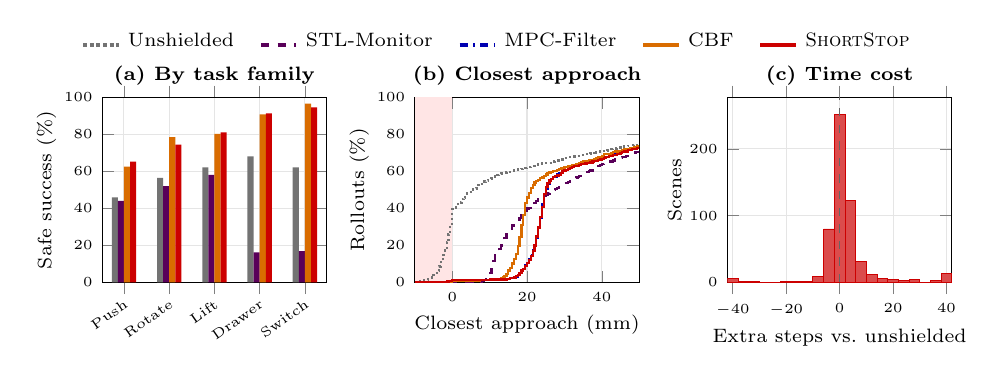
\begin{tikzpicture}
\pgfplotsset{every axis/.append style={scale only axis, width=2.85cm, height=2.35cm, tick label style={font=\tiny},
  label style={font=\scriptsize}, title style={font=\scriptsize\bfseries, yshift=-1.2ex},
  grid=major, grid style={gray!20}, ylabel shift=-4pt, xlabel shift=-2pt}}
\begin{axis}[name=a, ybar=0pt, bar width=2.2pt, ymin=0, ymax=100, ylabel={Safe success (\%)},
  symbolic x coords={push,rotate,lift,drawer,switch}, xtick=data,
  xticklabels={Push,Rotate,Lift,Drawer,Switch},
  xticklabel style={font=\tiny, rotate=35, anchor=north east, inner sep=1pt}, enlarge x limits=0.12,
  title={(a) By task family}]
\addplot[fill=black!55, draw=none] coordinates {(push,45.9) (rotate,56.5) (lift,62.2) (drawer,68.1) (switch,62.2)};
\addplot[fill=violet!70!black, draw=none] coordinates {(push,44.1) (rotate,52.0) (lift,58.1) (drawer,16.2) (switch,16.9)};
\addplot[fill=orange!85!black, draw=none] coordinates {(push,62.6) (rotate,78.5) (lift,80.2) (drawer,90.8) (switch,96.6)};
\addplot[fill=red!80!black, draw=none] coordinates {(push,65.3) (rotate,74.4) (lift,81.1) (drawer,91.4) (switch,94.6)};
\end{axis}
\begin{axis}[name=b, at={(a.south east)}, anchor=south west, xshift=1.12cm, xmin=-10, xmax=50, ymin=0, ymax=100,
  xlabel={Closest approach (mm)}, ylabel={Rollouts (\%)},
  title={(b) Closest approach}]
\fill[red!10] (axis cs:-10,0) rectangle (axis cs:0,100);
\addplot[black!55, densely dotted, line width=0.8pt, const plot, mark=none] coordinates {(-10.00,0.20) (-9.50,0.20) (-9.00,0.20) (-8.50,0.50) (-8.00,0.50) (-7.50,1.20) (-7.00,1.30) (-6.50,1.60) (-6.00,2.40) (-5.50,3.00) (-5.00,4.10) (-4.50,5.00) (-4.00,6.20) (-3.50,8.60) (-3.00,11.80) (-2.50,14.90) (-2.00,17.40) (-1.50,21.90) (-1.00,25.90) (-0.50,30.90) (0.00,39.70) (0.50,40.40) (1.00,41.30) (1.50,42.20) (2.00,43.20) (2.50,44.90) (3.00,45.80) (3.50,47.00) (4.00,48.00) (4.50,48.70) (5.00,49.20) (5.50,50.30) (6.00,50.70) (6.50,51.70) (7.00,52.50) (7.50,53.30) (8.00,53.90) (8.50,54.50) (9.00,55.10) (9.50,55.40) (10.00,55.80) (10.50,56.20) (11.00,57.00) (11.50,57.40) (12.00,58.20) (12.50,58.50) (13.00,58.90) (13.50,59.00) (14.00,59.20) (14.50,59.50) (15.00,59.70) (15.50,59.80) (16.00,60.00) (16.50,60.50) (17.00,60.60) (17.50,61.00) (18.00,61.10) (18.50,61.20) (19.00,61.40) (19.50,61.80) (20.00,62.00) (20.50,62.20) (21.00,62.60) (21.50,62.90) (22.00,63.40) (22.50,63.50) (23.00,63.80) (23.50,64.10) (24.00,64.30) (24.50,64.50) (25.00,64.60) (25.50,64.60) (26.00,64.60) (26.50,64.70) (27.00,65.30) (27.50,65.70) (28.00,65.90) (28.50,66.10) (29.00,66.40) (29.50,66.80) (30.00,67.10) (30.50,67.30) (31.00,67.60) (31.50,67.70) (32.00,67.90) (32.50,68.00) (33.00,68.40) (33.50,68.40) (34.00,68.50) (34.50,68.70) (35.00,69.00) (35.50,69.30) (36.00,69.50) (36.50,69.60) (37.00,69.70) (37.50,69.90) (38.00,70.10) (38.50,70.20) (39.00,70.50) (39.50,70.70) (40.00,71.00) (40.50,71.20) (41.00,71.20) (41.50,71.50) (42.00,71.70) (42.50,71.90) (43.00,72.10) (43.50,72.40) (44.00,72.80) (44.50,72.80) (45.00,72.90) (45.50,73.40) (46.00,73.50) (46.50,73.70) (47.00,73.90) (47.50,74.00) (48.00,74.10) (48.50,74.40) (49.00,74.40) (49.50,74.40) (50.00,74.60)};
\addplot[violet!70!black, dashed, line width=0.8pt, const plot, mark=none] coordinates {(-10.00,0.00) (-9.50,0.00) (-9.00,0.00) (-8.50,0.00) (-8.00,0.00) (-7.50,0.00) (-7.00,0.00) (-6.50,0.00) (-6.00,0.00) (-5.50,0.00) (-5.00,0.00) (-4.50,0.00) (-4.00,0.00) (-3.50,0.00) (-3.00,0.00) (-2.50,0.00) (-2.00,0.00) (-1.50,0.00) (-1.00,0.00) (-0.50,0.00) (0.00,0.00) (0.50,0.00) (1.00,0.00) (1.50,0.00) (2.00,0.00) (2.50,0.00) (3.00,0.00) (3.50,0.00) (4.00,0.00) (4.50,0.00) (5.00,0.00) (5.50,0.00) (6.00,0.00) (6.50,0.10) (7.00,0.20) (7.50,0.50) (8.00,0.80) (8.50,1.10) (9.00,1.80) (9.50,3.00) (10.00,5.00) (10.50,8.50) (11.00,11.60) (11.50,14.60) (12.00,15.90) (12.50,17.90) (13.00,19.90) (13.50,22.10) (14.00,24.10) (14.50,26.10) (15.00,27.90) (15.50,29.00) (16.00,30.80) (16.50,31.80) (17.00,32.60) (17.50,33.90) (18.00,35.00) (18.50,36.10) (19.00,37.50) (19.50,38.50) (20.00,39.90) (20.50,40.20) (21.00,41.10) (21.50,41.60) (22.00,43.10) (22.50,43.80) (23.00,44.80) (23.50,45.10) (24.00,45.70) (24.50,46.60) (25.00,47.30) (25.50,48.10) (26.00,48.60) (26.50,49.20) (27.00,50.00) (27.50,50.30) (28.00,51.00) (28.50,51.60) (29.00,52.00) (29.50,53.00) (30.00,53.60) (30.50,53.80) (31.00,54.30) (31.50,55.00) (32.00,55.90) (32.50,56.40) (33.00,56.70) (33.50,56.90) (34.00,57.50) (34.50,58.40) (35.00,58.70) (35.50,59.00) (36.00,59.70) (36.50,60.10) (37.00,60.50) (37.50,61.20) (38.00,61.70) (38.50,61.90) (39.00,62.70) (39.50,63.30) (40.00,63.80) (40.50,64.30) (41.00,64.60) (41.50,64.80) (42.00,65.30) (42.50,65.30) (43.00,65.90) (43.50,66.50) (44.00,66.80) (44.50,66.80) (45.00,67.50) (45.50,67.80) (46.00,67.90) (46.50,68.20) (47.00,69.10) (47.50,69.40) (48.00,69.70) (48.50,70.10) (49.00,70.40) (49.50,70.60) (50.00,70.80)};
\addplot[blue!70!black, dashdotted, line width=0.8pt, const plot, mark=none] coordinates {(-10.00,0.10) (-9.50,0.10) (-9.00,0.10) (-8.50,0.10) (-8.00,0.10) (-7.50,0.10) (-7.00,0.10) (-6.50,0.10) (-6.00,0.20) (-5.50,0.20) (-5.00,0.20) (-4.50,0.20) (-4.00,0.30) (-3.50,0.30) (-3.00,0.30) (-2.50,0.30) (-2.00,0.30) (-1.50,0.50) (-1.00,0.70) (-0.50,0.80) (0.00,1.00) (0.50,1.10) (1.00,1.10) (1.50,1.10) (2.00,1.20) (2.50,1.20) (3.00,1.20) (3.50,1.20) (4.00,1.30) (4.50,1.30) (5.00,1.40) (5.50,1.40) (6.00,1.40) (6.50,1.40) (7.00,1.40) (7.50,1.50) (8.00,1.50) (8.50,1.50) (9.00,1.50) (9.50,1.50) (10.00,1.50) (10.50,1.60) (11.00,1.60) (11.50,1.60) (12.00,1.60) (12.50,1.60) (13.00,1.70) (13.50,1.80) (14.00,1.80) (14.50,1.90) (15.00,1.90) (15.50,2.40) (16.00,2.60) (16.50,2.80) (17.00,2.90) (17.50,4.10) (18.00,5.10) (18.50,5.80) (19.00,7.30) (19.50,9.50) (20.00,10.70) (20.50,12.50) (21.00,14.80) (21.50,17.40) (22.00,19.90) (22.50,24.20) (23.00,29.60) (23.50,34.90) (24.00,42.10) (24.50,46.80) (25.00,50.60) (25.50,53.10) (26.00,55.40) (26.50,56.60) (27.00,57.00) (27.50,57.20) (28.00,58.40) (28.50,58.80) (29.00,59.50) (29.50,60.50) (30.00,61.00) (30.50,61.10) (31.00,61.30) (31.50,61.70) (32.00,62.30) (32.50,62.50) (33.00,62.70) (33.50,63.00) (34.00,63.40) (34.50,63.70) (35.00,63.90) (35.50,64.40) (36.00,64.50) (36.50,64.80) (37.00,65.20) (37.50,65.60) (38.00,66.00) (38.50,66.30) (39.00,66.90) (39.50,66.90) (40.00,67.30) (40.50,67.80) (41.00,67.80) (41.50,67.90) (42.00,68.10) (42.50,68.70) (43.00,69.20) (43.50,69.40) (44.00,69.40) (44.50,69.50) (45.00,69.80) (45.50,70.60) (46.00,70.80) (46.50,71.40) (47.00,71.40) (47.50,71.80) (48.00,72.10) (48.50,72.40) (49.00,72.60) (49.50,72.60) (50.00,73.20)};
\addplot[orange!85!black, solid, line width=0.8pt, const plot, mark=none] coordinates {(-10.00,0.00) (-9.50,0.00) (-9.00,0.00) (-8.50,0.00) (-8.00,0.00) (-7.50,0.00) (-7.00,0.00) (-6.50,0.00) (-6.00,0.00) (-5.50,0.00) (-5.00,0.00) (-4.50,0.00) (-4.00,0.00) (-3.50,0.10) (-3.00,0.10) (-2.50,0.10) (-2.00,0.10) (-1.50,0.20) (-1.00,0.40) (-0.50,0.50) (0.00,0.70) (0.50,0.70) (1.00,0.70) (1.50,0.70) (2.00,0.70) (2.50,0.70) (3.00,0.70) (3.50,0.70) (4.00,0.70) (4.50,0.80) (5.00,0.90) (5.50,0.90) (6.00,0.90) (6.50,1.00) (7.00,1.00) (7.50,1.10) (8.00,1.10) (8.50,1.20) (9.00,1.30) (9.50,1.30) (10.00,1.30) (10.50,1.40) (11.00,1.50) (11.50,1.60) (12.00,1.70) (12.50,2.00) (13.00,2.20) (13.50,2.90) (14.00,3.50) (14.50,4.40) (15.00,6.40) (15.50,7.70) (16.00,10.20) (16.50,12.50) (17.00,15.30) (17.50,19.70) (18.00,24.60) (18.50,31.20) (19.00,36.50) (19.50,42.80) (20.00,45.90) (20.50,48.50) (21.00,51.20) (21.50,52.60) (22.00,54.00) (22.50,54.80) (23.00,55.50) (23.50,56.30) (24.00,56.70) (24.50,57.30) (25.00,58.30) (25.50,59.10) (26.00,59.40) (26.50,59.80) (27.00,60.20) (27.50,60.20) (28.00,60.70) (28.50,61.10) (29.00,61.60) (29.50,62.00) (30.00,62.40) (30.50,62.50) (31.00,62.80) (31.50,63.00) (32.00,63.30) (32.50,63.50) (33.00,63.80) (33.50,63.90) (34.00,64.20) (34.50,64.80) (35.00,65.30) (35.50,65.60) (36.00,65.80) (36.50,66.00) (37.00,66.10) (37.50,66.30) (38.00,66.70) (38.50,67.40) (39.00,67.70) (39.50,67.90) (40.00,68.20) (40.50,69.30) (41.00,69.30) (41.50,69.50) (42.00,69.60) (42.50,70.00) (43.00,70.50) (43.50,70.80) (44.00,70.80) (44.50,70.90) (45.00,71.00) (45.50,71.70) (46.00,71.80) (46.50,72.10) (47.00,72.30) (47.50,72.40) (48.00,72.70) (48.50,73.10) (49.00,73.20) (49.50,73.40) (50.00,73.50)};
\addplot[red!80!black, solid, line width=0.8pt, const plot, mark=none] coordinates {(-10.00,0.00) (-9.50,0.00) (-9.00,0.00) (-8.50,0.00) (-8.00,0.00) (-7.50,0.00) (-7.00,0.00) (-6.50,0.10) (-6.00,0.10) (-5.50,0.10) (-5.00,0.10) (-4.50,0.10) (-4.00,0.20) (-3.50,0.30) (-3.00,0.30) (-2.50,0.30) (-2.00,0.30) (-1.50,0.50) (-1.00,0.80) (-0.50,0.90) (0.00,1.10) (0.50,1.10) (1.00,1.10) (1.50,1.10) (2.00,1.10) (2.50,1.10) (3.00,1.10) (3.50,1.10) (4.00,1.10) (4.50,1.10) (5.00,1.10) (5.50,1.30) (6.00,1.40) (6.50,1.40) (7.00,1.40) (7.50,1.40) (8.00,1.50) (8.50,1.50) (9.00,1.50) (9.50,1.50) (10.00,1.60) (10.50,1.60) (11.00,1.60) (11.50,1.60) (12.00,1.60) (12.50,1.60) (13.00,1.60) (13.50,1.60) (14.00,1.60) (14.50,1.80) (15.00,1.90) (15.50,2.20) (16.00,2.50) (16.50,2.60) (17.00,3.30) (17.50,4.10) (18.00,5.20) (18.50,6.40) (19.00,7.40) (19.50,8.80) (20.00,10.30) (20.50,12.30) (21.00,14.20) (21.50,17.00) (22.00,20.00) (22.50,24.80) (23.00,29.70) (23.50,35.40) (24.00,40.70) (24.50,47.60) (25.00,51.50) (25.50,53.90) (26.00,55.10) (26.50,56.00) (27.00,56.80) (27.50,57.30) (28.00,57.80) (28.50,58.20) (29.00,59.00) (29.50,60.00) (30.00,60.50) (30.50,60.90) (31.00,61.30) (31.50,61.80) (32.00,62.30) (32.50,62.80) (33.00,62.90) (33.50,63.00) (34.00,63.30) (34.50,64.00) (35.00,64.10) (35.50,64.20) (36.00,64.60) (36.50,64.60) (37.00,64.80) (37.50,65.30) (38.00,65.70) (38.50,65.80) (39.00,66.30) (39.50,66.40) (40.00,66.80) (40.50,67.40) (41.00,67.60) (41.50,67.90) (42.00,68.10) (42.50,68.30) (43.00,68.70) (43.50,69.00) (44.00,69.40) (44.50,69.50) (45.00,69.90) (45.50,70.30) (46.00,70.70) (46.50,70.80) (47.00,71.40) (47.50,71.70) (48.00,71.90) (48.50,72.20) (49.00,72.30) (49.50,72.50) (50.00,72.60)};
\end{axis}
\begin{axis}[name=c, at={(b.south east)}, anchor=south west, xshift=1.12cm, ybar, bar width=4, ymin=0,
  xmin=-42, xmax=42, xtick={-40,-20,0,20,40},
  xlabel={Extra steps vs.\ unshielded}, ylabel={Scenes},
  title={(c) Time cost}]
\addplot[fill=red!80!black!70, draw=red!80!black, line width=0.3pt] coordinates {(-40,6) (-36,2) (-32,1) (-28,0) (-24,0) (-20,1) (-16,2) (-12,2) (-8,9) (-4,80) (0,252) (4,123) (8,31) (12,12) (16,6) (20,5) (24,3) (28,5) (32,0) (36,3) (40,14)};
\draw[black!60, dashed] (axis cs:0,\pgfkeysvalueof{/pgfplots/ymin}) -- (axis cs:0,\pgfkeysvalueof{/pgfplots/ymax});
\end{axis}
\matrix[matrix of nodes, anchor=south, font=\scriptsize, column sep=7pt, inner sep=1pt,
  nodes={anchor=west}] at ($(b.outer north)+(0,0.05)$) {
\tikz\draw[black!55, densely dotted, line width=1.4pt] (0,0) -- (0.45,0); Unshielded & \tikz\draw[violet!70!black, dashed, line width=1.4pt] (0,0) -- (0.45,0); STL-Monitor & \tikz\draw[blue!70!black, dashdotted, line width=1.4pt] (0,0) -- (0.45,0); MPC-Filter & \tikz\draw[orange!85!black, solid, line width=1.4pt] (0,0) -- (0.45,0); CBF & \tikz\draw[red!80!black, solid, line width=1.4pt] (0,0) -- (0.45,0); \sys{} \\
};
\end{tikzpicture}

\caption{Three views of the main run that Table~\ref{tab:main} does not show.
(a)~Safe success per task family (MPC-Filter, omitted, is within 4 points of
CBF). (b)~Cumulative share of rollouts by closest approach of the real arm
to an obstacle (shaded: collision). (c)~\sys{} minus unshielded steps on the
557 scenes all four methods complete, clipped at $\pm$40 steps.}
\label{fig:views}
\end{figure}

\subsection{Main Comparison}
Shielding improves both collision avoidance and task completion
(Table~\ref{tab:main}). Collisions fall from 39.7\% under unshielded
execution to 1.1\% ($-38.6$ percentage points, $p<0.001$), while safe
success rises from 58.4\% to 80.0\% ($+21.6$ points, $p<0.001$).
These gains describe scenes deliberately chosen to challenge the
unshielded policy through filter (iii). All filters face the same scenes.

In paired outcomes, \sys{} alone succeeds in 235 scenes and the
unshielded policy alone in 19. Of the 397 scenes with unshielded collisions, \sys{} completes
57.2\% safely (CBF 58.9\%, MPC 54.7\%). Most of the remaining scenes
time out. Intervention is frequent, affecting 52.9\% of proposals,
but only 11.1\% of decisions end in a hold.

\textbf{Task and clearance differences.} Contact requirements help explain
task variation (Fig.~\ref{fig:views}a). Pushing requires sustained contact
with a moving block near obstacles, limiting safe success to 62--65\%
across the three model-based filters. Drawer and switch
tasks reach 90--97\%. The drawer family includes drawer, slider and
push-into-drawer tasks, while switches operate a light-emitting diode
(LED) or lightbulb. STL-Monitor completes just 16\% and 17\% of these
two families: repeated rejection can prevent the contact needed to finish.
Neither \sys{} nor CBF leads on every task. Pushing favours \sys{}
(65.3\% against 62.6\%), whereas rotation favours CBF (78.5\% against 74.4\%).

The filters also keep the arm farther from obstacles
(Fig.~\ref{fig:views}b). With bands of 10--22~mm around the predicted arm
and a further 3~mm margin, the median closest approach is 25~mm for
\sys{} and MPC, or 21~mm for CBF. Fewer than 2\% of their rollouts
pass within 10~mm of an obstacle, compared with 56\% unshielded.
This extra clearance costs little execution time on the 557 scenes all
four methods complete safely: each has a median completion time of
66 steps. For \sys{}, the paired difference from unshielded is zero
at the median and within 10 steps in 90\% of scenes
(Fig.~\ref{fig:views}c). The main cost appears in scenes that stall.

\textbf{Comparison with model-based filters.} With the model, error bound,
margin and fallback held fixed, the three filters perform similarly.
The violation rate for \sys{} differs from CBF and MPC by $+0.4$ and $+0.1$ points
($p=0.21$ and $0.88$). For safe success, the difference from CBF is
$-0.3$ points ($p=0.76$, 33 vs.\ 36 discordant scenes), while the
$+1.5$ points over MPC ($p=0.0496$) do not survive Holm's correction.
All $p<0.001$ comparisons here remain significant after correction.
Conservatism cost follows the same pattern: our estimate is 1.8 points
[0.2, 3.5], CBF's is 2.5 [1.2, 3.9], and MPC's is 2.7 [1.3, 4.1],
with neither difference statistically significant ($p=0.43$ and $0.34$).
Thus the measured outcomes are comparable despite different correction rules.

STL-Monitor exposes the cost of frequent rejection. It records no
collisions, but rejects 93.6\% of decisions and leaves 60.2\% of scenes
unfinished. Relative to this monitor, \sys{} gains 40.2 safe-success
points ($p<0.001$, 407 vs.\ 5 discordant scenes) with 1.1 points more
violations. Differences in tube, margin and repair prevent attribution to repair
alone, which Sect.~\ref{sec:analysis} isolates. Conf-Thresh, meanwhile, behaves much like
the unshielded policy: disagreement among samples fails to flag unsafe motions here.

\textbf{Latency and continued progress.} Similar outcomes conceal different
computational costs. \sys{} adds a median 56~ms per decision, including
27~ms for the progress score, with p99 328~ms and maximum 408~ms.
MPC handles feasible chunks quickly (median 13~ms), but its p99 reaches
652~ms and its maximum 1.36~s. CBF varies less (median 101~ms, maximum
309~ms), with one QP solved per executed row in our Python implementation.
MDT inference adds a median 104~ms on our graphics processing unit (GPU).
The measured median full decision takes about 165~ms, exceeding the
133~ms available for $r=4$ steps at 30~Hz. This mismatch makes inference
delay part of the execution problem (Remark~\ref{rem:delay}).
A feasible QP can often produce a small motion when our repair fails,
helping explain the higher fallback rate of \sys{} (11.1\% vs.\ MPC's
5.6\% and CBF's 2.7\%). Despite this difference, all three time out in
19--21\% of scenes.

\subsection{Empirical Soundness of the Certificate}\label{sec:soundness}
A passive audit compares predicted bands with actual motion on the first
300 test scenes. It reproduces all 300 main-run outcomes while examining
tube coverage and fallback safety
(Assumptions~\ref{as:tube} and~\ref{as:fb}). Across 41{,}899 certified
rows, the arm leaves its tube in 0.10\%
(0.06, 0.08, 0.11 and 0.17\% at $k=1,\dots,4$), below the $\delta_k$ levels
in Sect.~\ref{sec:setup}. The 99th-percentile errors, 6.0--14.4~mm, remain
below their corresponding radii. Actual robustness falls below the
certificate in 0.02\% of rows. Assumption~\ref{as:stl} holds by construction.
Across all 1000 scenes, none of our 11, MPC's 10 or CBF's 7 collisions
occurs during fallback.

The rare failures reveal a specific weakness. Both collisions in the
audited subset occur during certified motion, when pushing or lifting
produces errors of 22 and 51~mm against radii of 14.7 and 18.5~mm.
Contact also dominates failures in the full test set: lifting a block
from the slider accounts for 9 of our 11 collisions and 6 of CBF's 7.
These contact effects were absent from the obstacle-free calibration.

\begin{table}[t]
\caption{Component ablation on the first 300 test scenes ($H = 4$). Each
rung adds one component. Last column ($\Delta$): paired safe-success change against
the rung above (points, $p$). Lat.: p95 latency in ms over these 300 scenes
(Table~\ref{tab:main} pools all 1000).}\label{tab:ablation}
\centering\scriptsize\setlength{\tabcolsep}{2.5pt}
\begin{tabular}{@{}l>{\raggedright\arraybackslash}p{3.1cm}cccccc@{}}
\toprule
Rung & Configuration & Safe succ.\ (\%) & Viol. & Activ. & Fallb. & Lat. & $\Delta$ vs.\ above \\
\midrule
\tablerows{tables/ablation.tex}
\bottomrule
\end{tabular}
\end{table}

\subsection{Inference Delay}\label{sec:delay}
We test Remark~\ref{rem:delay} on the first 200 test scenes with
$d \in \{1,2,3\}$, where the next chunk is computed while the committed rows
run~\cite{black2025rtc}. Each filter runs in a \emph{naive} mode (the final
configuration with $H = 4$, unaware of the delay) and in an \emph{aware}
mode ($H = 4 + d$, committed rows fixed). CBF has no horizon, and its aware
mode leaves the committed rows uncorrected and filters the rows after
them. Nothing is re-tuned (Table~\ref{tab:delay}).

\begin{table}[t]
\caption{Inference delay $d$ on the first 200 test scenes (\%). Naive:
$H{=}4$. Aware: $H{=}4{+}d$ (CBF: rows after the committed ones). Last two columns: paired difference in points
with bootstrap $p$.}\label{tab:delay}
\centering\scriptsize\setlength{\tabcolsep}{4pt}
\begin{tabular}{@{}clcccc@{}}
\toprule
 & & \multicolumn{2}{c}{Safe succ.\ / viol.} & \multicolumn{2}{c}{Aware $-$ naive ($p$)} \\
\cmidrule(lr){3-4}\cmidrule(l){5-6}
$d$ & Method & Naive & Aware & Safe succ. & Viol. \\
\midrule
\tablerows{tables/delay.tex}
\bottomrule
\end{tabular}
\end{table}

Committed rows become consequential once the delay reaches $d\ge2$:
all three filters benefit substantially from accounting for them
(Table~\ref{tab:delay}). Without this adjustment, violations under \sys{}
rise from 2.0\% to 14.0\% to 31.5\% as $d$ increases, approaching the
unshielded rate of 44.5\%. Certifying $H=r+d$ keeps the corresponding
rates at 0.5\%, 0.5\% and 0.0\%.
The reductions at $d=2$ and $3$ are 13.5 and 31.5 points ($p<0.001$).
MPC and CBF show the same pattern, with aware violation rates at most 1.5\%.
Longer certification costs 2--6 safe-success points at $d\le2$. At $d=3$,
where collisions dominate the naive mode, the aware mode has higher safe
success (72.0\% vs.\ 68.5\%, $p=0.33$). Our aware safe success ranges from
72.0\% to 74.5\%, within $\pm4.5$ points of the baselines.

%=====================================================================
\section{Analysis and Ablations}\label{sec:analysis}

To separate repair from the other design choices, we build the shield
one component at a time on the first 300 scenes (Table~\ref{tab:ablation}).
Starting with the unshielded policy (L0), we certify one sample and hold
on rejection (L1), then draw $K=4$ samples and take the first certified
one (L2). Ranking by $g(a)$ gives L3. Adding repair yields the full method, L4.

Certification alone removes the observed collisions: L1 reduces violations
from 41.7\% to 0.0\%. But the robot holds in 95\% of decisions, times out
in 217 of 300 scenes, and completes only 27.7\% safely. Sampling more
chunks changes little (L2, $+0.0$ points, 1 vs.\ 1 discordant scene), as
does ranking them (L3, $+1.0$ point, 6 vs.\ 3). MDT's samples are nearly
identical and tend to fail the same check. Repair changes the motions
available for execution, adding 50.7 safe-success points (152 scenes won,
none lost, $p<0.001$) and reducing fallback from 95.2\% to 14.6\%. The two
collisions introduced in L4 (0.7\%) are the contact cases discussed in
Sect.~\ref{sec:soundness}.

\textbf{Horizon.}\label{sec:horizon} Without delay, certifying beyond the
executed prefix offers more look-ahead but requires wider bands.
We compare $H\in\{4,6,8\}$ on the same 300 scenes, covering the executed
rows while staying within our calibrated range. Validation safe success is 75.0, 72.5 and 72.5\%.
On test, extending $H$ to 6 and 8 reduces safe success to 73.3\% and
70.7\%, losses of 6.0 and 8.7 points ($p<0.001$ each, 18 vs.\ 0 and
29 vs.\ 3 discordant scenes). Violations remain within one scene
(0.7, 0.3 and 0.7\%). Fallback rises from 14.6\% to 18.4\% and 15.9\%,
and p95 latency from 253 to 286 and 299~ms. These results are consistent
with the conservatism bound in Proposition~\ref{prop:conservatism}.
Among the tested settings, $H=r$ works best without delay, while the
delay study supports $H=r+d$.

%=====================================================================
\section{Discussion and Limitations}\label{sec:limits}

\textbf{Benchmark scope.} Static-obstacle avoidance reduces our STL check
to set invariance, a setting well suited to a CBF. Comparable performance
here leaves open whether richer temporal specifications would favour our
formulation. The low proposal diversity also matters: MDT endpoints lie
only 0.7~mm from their centroid at the median, limiting what additional
samples can offer. Our kinematic model captures arm geometry but omits
the contact effects associated with residual collisions.

All experiments use one simulator, one policy and one rollout per scene.
The 1000 paired scenes leave policy-seed variation unmeasured. Hardware
evaluation and comparison with PACS~\cite{roemer2026pacs}, which brakes
along the proposed path, remain to be done. The deterministic
simulator also leaves nonzero $\bar w$ untested.

\textbf{Implementation limits.} Joint limits are checked on the nominal
path but omitted from our obstacle-repair objective. MPC and CBF include
them in their QPs. Affected decisions (3\%) fall back, costing at most
0.4 safe-success points. Repairs and contact can break exchangeability, while long episodes weaken
the union bound. The observed escape rate of 0.10\% concerns sampled
states, leaving motion between 30~Hz samples uncovered. The 11\% fallback
rate also limits \emph{liveness}, or continued task progress.

%=====================================================================
\section{Conclusion}
\sys{} uses failed clearance checks to repair the short-term motions
of a frozen generative policy. Its safety guarantee depends on tube
coverage, observed in 99.9\% of audited steps. On CALVIN, collisions fall
by 97\% relative to unshielded execution and safe success rises by
21.6 points, with outcomes comparable to filters sharing our model.
The delay study yields a practical requirement: certification must follow
the execution schedule. Accounting for the $H\ge r+d$ rows keeps every
tested filter's violation rate at or below 1.5\%. Temporal specifications,
comparison with PACS, and hardware evaluation are the next tests of how
far these findings extend.

\textbf{Code and data availability.} Code, frozen scenes, calibration data
and all rollouts are available at \url{https://github.com/congtul/shortstop-calvin}.

\begin{credits}
\subsubsection{\ackname}
We acknowledge Ho Chi Minh City University of Technology (HCMUT), VNU-HCM
for supporting this study.
\end{credits}

\bibliographystyle{splncs04}
\bibliography{refs,refs-new}

\end{document}
